\chapter{Korisnički računi}

\section{Kreiranje korisničkog računa - registracija}

Na sljedećoj slici je prikazana stranica koja omogućava registraciju korisnika na sistem:

\begin{center}
    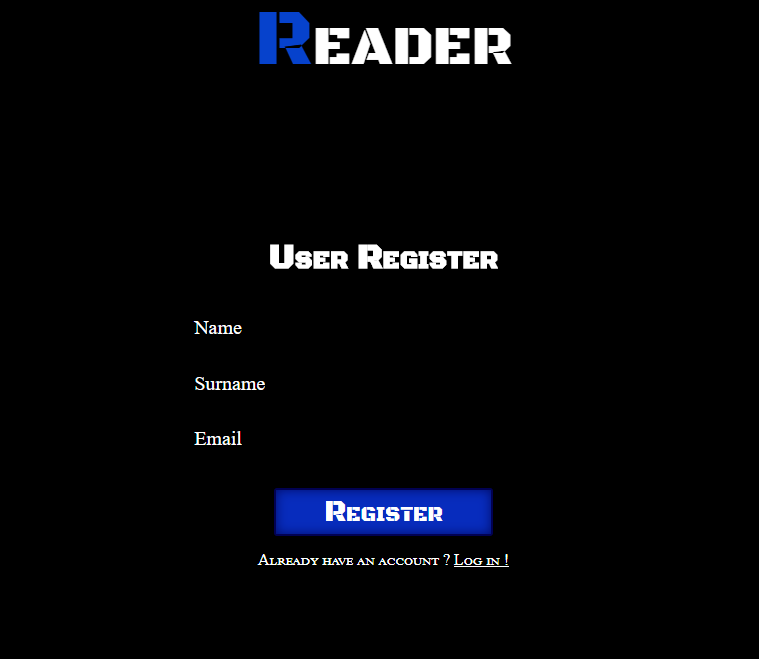
\includegraphics[scale=0.6]{images/Registracija.png}
    \captionof{figure}{Registracija korisnika}
\end{center}

Na stranici se nalaze tri polja za unos teksta:
\begin{enumerate}
    \item Name - polje za unos imena korisnika koje ne može ostati prazno
    \item Surname - polje za unos prezimena korisnika
    \item Email - polje za unos mail-a korisnika koje mora predstavljati validnu mail adresu, s obzirom da se prilikom registracije obavlja verifikacija preko unesene mail adrese
\end{enumerate}

Dugmetom \texttt{Register} se potvrđuju uneseni podaci nakon čega započinje proces registracije korisnika. Ispod dugmeta, nalazi se link (\texttt{Already have an account? Log In!}) koji vraća korisnika na stranicu za prijavu.

\section{Prijava na sistem - Log In}

Sljedećom slikom je prikazan izgled stranice prilikom prijave korisnika na sistem:

\begin{center}
    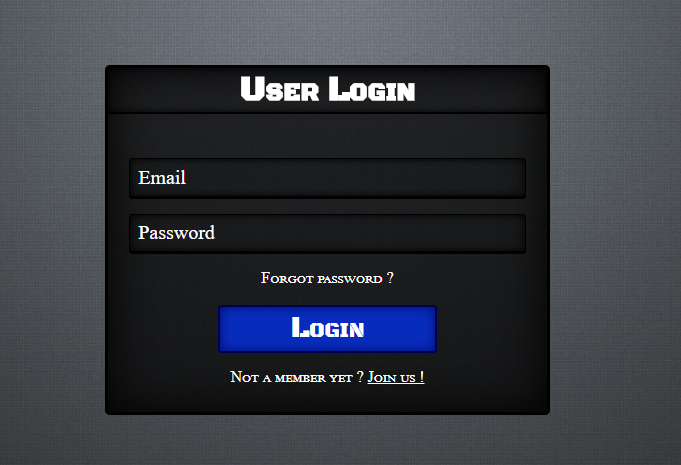
\includegraphics[scale=0.6]{images/Login.png}
    \captionof{figure}{Prijava korisnika na sistem}
\end{center}

Stranica sadrži dva polja za unos teksta:
\begin{enumerate}
    \item Email - polje za unos mail-a, unesenog prilikom registracije korisnika
    \item Password - polje za unos lozinke
\end{enumerate}

Klikom na link \texttt{Forgot Password?} korisnik započinje postupak dobijanja nove lozinke za pristup sistemu. Dugmetom \texttt{Login} potvrđuju se uneseni podaci i prikazuje se odgovarajuća stranica sistema (ukoliko su podaci ispravni). Klikom na link ispod dugmeta (\texttt{Not a member yet? Join us!}) prikazuje se stranica za registraciju korisnika.

\newpage
\section{Modifikacija korisničkih podataka}

Sljedećom slikom je prikazan izgled stranice za modifikaciju korisničkih podataka:

\begin{center}
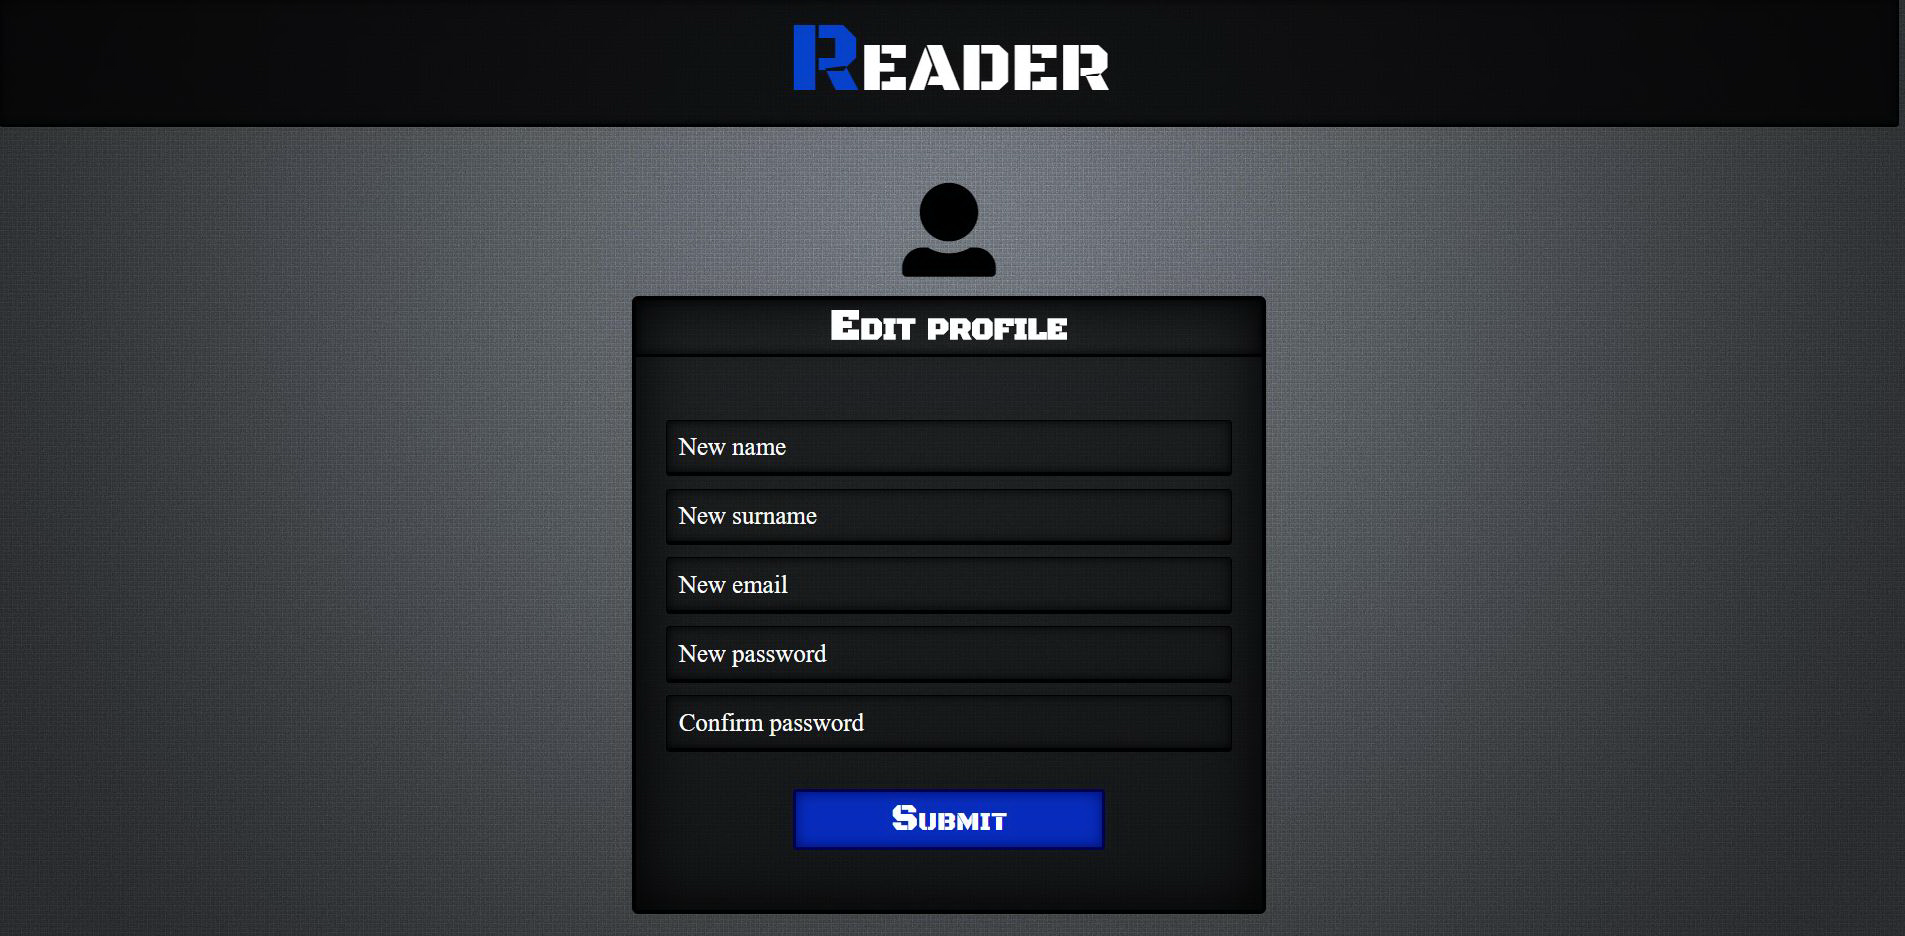
\includegraphics[scale=0.2]{images/ModifikacijaKorisnickihPodataka.png}
\captionof{figure}{Modifikacija korisničkog računa}
\end{center}

Stranica sadrži sljedeća polja za unos teksta:
\begin{enumerate}
\item New name - polje za unos novog imena korisnika
\item New surname - polje za unos novog prezimena korisnika
\item New email - polje za unos novog mail-a, ili starog ukoliko želi zadržati stari mail
\item New password - polje za unos novog passworda, ili starog ukoliko želi zadržati stari
\item Confirm password - polje u koje korisnik unosi isti password kao u prethodnom polju za potvrdu, vrši se provjera na jednakost ova dva polja
\end{enumerate}

Klikom na dugme \texttt{Submit} korisnik potvrđuje izmjenu podataka. Korisnik dobija poruku o uspješnoj izmjeni i vrši se redirekcija na početnu stranicu.

\newpage
\section{Brisanje korisničkog računa}

Sljedećom slikom je prikazan izgled stranice za brisanje korisničkog računa:

\begin{center}
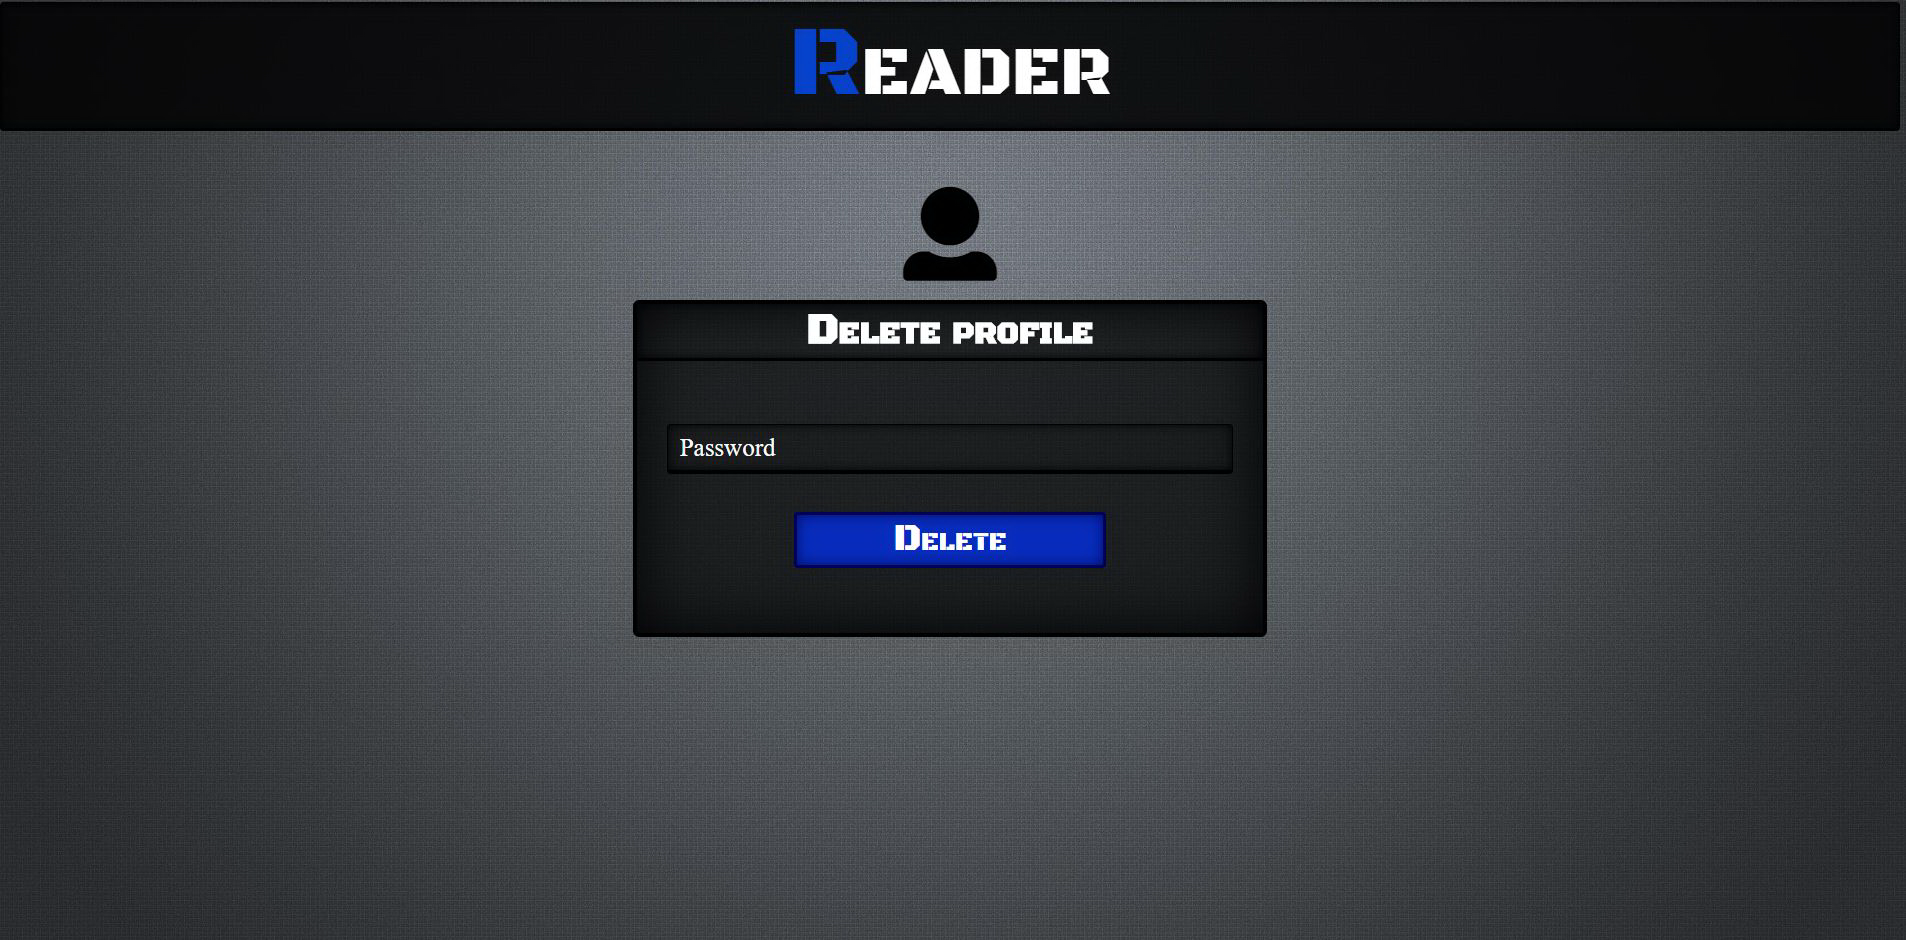
\includegraphics[scale=0.2]{images/BrisanjeKorisnickogRacuna.png}
\captionof{figure}{Brisanje korisničkog računa}
\end{center}

Stranica sadrži jedno polje za unos teksta:
\begin{enumerate}
\item Password - polje za unos passworda za autentifikaciju korisnika
\end{enumerate}
Klikom na dugme \texttt{Delete} korisnik potvrđuje brisanje korisničkog računa. Korisnički račun se briše, a korisnik dobija poruku o uspješnom brisanju i vrši se redirekcija na početnu stranicu aplikacije, gdje korisnik može kreirati novi račun.

\newpage
\section{Glavna stranica}

Nakon uspješnog prijavljivanja na račun, korisniku se prikazuje njegova početna stranica, odnosno glavna stranica aplikacije, koja je prikazana na narednoj slici.

\begin{center}
    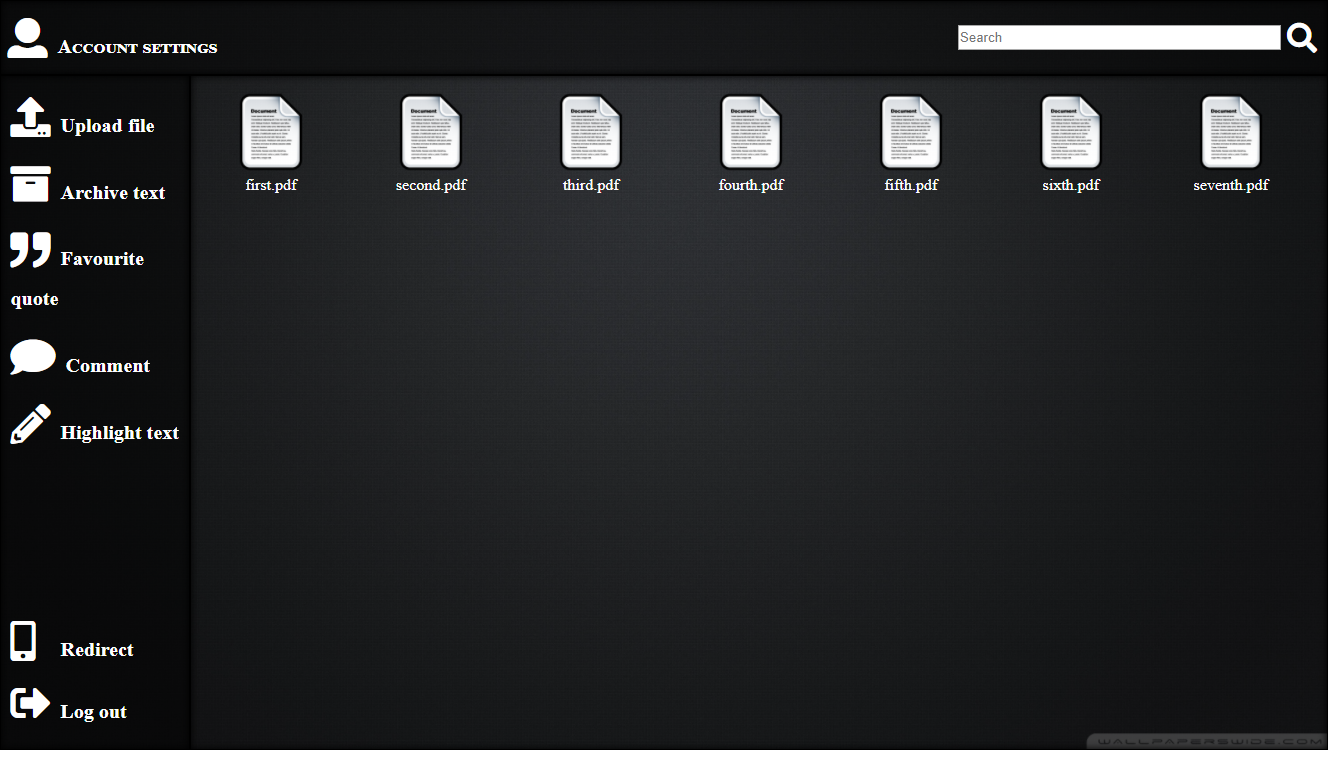
\includegraphics[scale=0.45]{images/Home.png}
    \captionof{figure}{Glavna stranica}
\end{center}

Prikaz stranice možemo podijeliti na četiri sekcije: 
\begin{enumerate}
    \item \textit{Zaglavlje} u kojem se nalazi dugme koje otvara stranicu za modifikaciju podataka, te polje za pretragu \textit{upload}-ovanih dokumenata
    \item \textit{Centralni dio} u kojem su prikazani dokumenti koje je korisnik ranije \textit{upload}-ovao
    \item \textit{Desna sekcija} stranice gdje se nalaze osnovne funkcionalnosti koje korisnik primjenjuje nad dokumentom
    \item \textit{Podnožje} sa opcijama \iextit{Log Out}-a, te linkom za instalaciju mobilne verzije aplikacije
\end{enumerate}

Upload dokumenta se vrši klikom na dugme \textit{Upload file}, nakon čega se otvara prozor sa lokalnim direktorijem, te izabere željeni dokument. Dokument je zatim vidljiv u centralnom dijelu interfejsa.\\ Upisivanjem ključne riječi u polje za pretragu, filtriraju se dokumenti prikazani u centralnom dijelu i na taj način omogućava korisniku brži i lakši pronalazak traženog dokumenta. Neke od opcija sa desne strane korisničkog interfejsa imaju dvojaku primjenu u zavisnosti da li su u centralnom dijelu prikazani svi upload-ovani dokumenti ili je otvoren jedan od njih. Prvo će biti opisan slučaj sa prikazom svih dokumenata na profilu. Pritiskom na dugme \textit{Achive text}, u ovom slučaju, prikazuju se svi prethodno arhivirani citati, dok dugme \textit{Favourite quote} otvara omiljene citate korisnika. Preostale dvije opcije je moguće primijeniti tek nakon otvaranja dokumenta. \\ Otvaranjem dokumenta, moguće je iskoristiti dugme \textit{Archive text} za arhiviranje novog isječka, te \textit{Favourite quote} za izdvajanje novog omiljenog citata. Obje opcije se izvršavaju tako što se obilježi željeni citat i zatim pritisne na odgovarajuću opciju. Prilikom čitanja dokumenta također je moguće ostavljati komentare pritiskom na dugme \textit{Comment} i na željeno mjesto u dokumentu. Na ovaj način je omogućeno stvaranje bilješki prilikom čitanja, što olakšava kasnije snalaženje u dokumentu. \\ \textit{Highlight text} prikazuje moguće opcije za odabir vizualnog načina označavanja citata.

